\section{eo\-Variable\-Pareto\-Traits Class Reference}
\label{classeo_variable_pareto_traits}\index{eoVariableParetoTraits@{eoVariableParetoTraits}}
eo\-Variable\-Pareto\-Traits : an {\bf eo\-Pareto\-Fitness\-Traits}{\rm (p.\,\pageref{classeo_pareto_fitness_traits})} whose characteristics can be set at run-time (nb objectives and min/max's) Why bother? For didactical purposes (and EASEA implementation :-)  


{\tt \#include $<$eo\-Pareto\-Fitness.h$>$}

Inheritance diagram for eo\-Variable\-Pareto\-Traits::\begin{figure}[H]
\begin{center}
\leavevmode
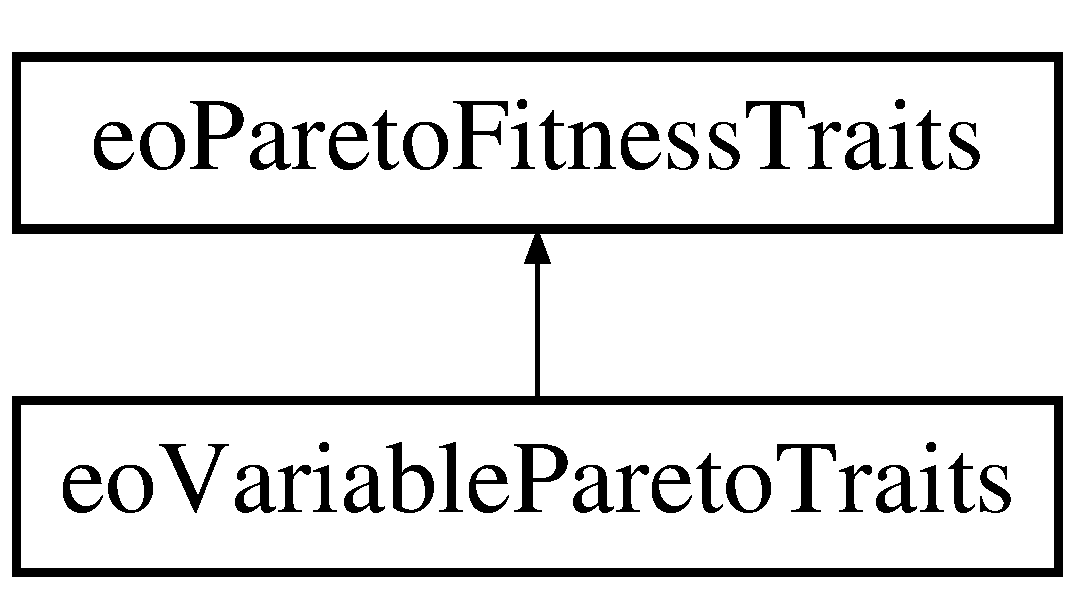
\includegraphics[height=2cm]{classeo_variable_pareto_traits}
\end{center}
\end{figure}
\subsection*{Static Public Member Functions}
\begin{CompactItemize}
\item 
void {\bf set\-Up} (unsigned \_\-n, std::vector$<$ bool $>$ \&\_\-b)\label{classeo_variable_pareto_traits_e0}

\begin{CompactList}\small\item\em setting the static stuff \item\end{CompactList}\item 
unsigned {\bf n\-Objectives} ()\label{classeo_variable_pareto_traits_e1}

\begin{CompactList}\small\item\em the accessors \item\end{CompactList}\item 
bool {\bf maximizing} (unsigned \_\-i)\label{classeo_variable_pareto_traits_e2}

\end{CompactItemize}
\subsection*{Static Private Attributes}
\begin{CompactItemize}
\item 
unsigned {\bf n\-Obj}\label{classeo_variable_pareto_traits_v0}

\item 
std::vector$<$ bool $>$ {\bf b\-Obj}\label{classeo_variable_pareto_traits_v1}

\end{CompactItemize}


\subsection{Detailed Description}
eo\-Variable\-Pareto\-Traits : an {\bf eo\-Pareto\-Fitness\-Traits}{\rm (p.\,\pageref{classeo_pareto_fitness_traits})} whose characteristics can be set at run-time (nb objectives and min/max's) Why bother? For didactical purposes (and EASEA implementation :-) 



Definition at line 56 of file eo\-Pareto\-Fitness.h.

The documentation for this class was generated from the following files:\begin{CompactItemize}
\item 
eo\-Pareto\-Fitness.h\item 
eo\-Pareto\-Fitness.cpp\end{CompactItemize}
